\chapter{Startup}

This section describes the function and operation of the control elements located on the machine’s control panel. For more details, refer to \textbf{Section 10.7}.

\section{Starting the Machine and the Control}

\begin{enumerate}
    \item Switch on the \textbf{main switch} in the machine's electrical cabinet to the \textbf{"On"} position.
    
    \item Once the \textbf{MANUAL} screen appears on the display:
    \begin{enumerate}
        \iconitem{Press the illuminated button \textbf{HYDRAULIC ON} to activate the machine’s hydraulic and electrical systems.}{hydraulics_on.jpg}
        \item Immediately after startup, the machine automatically checks the \textbf{EMERGENCY STOP} circuit.
        \iconitem {Within \textbf{5 seconds} after startup, press the illuminated button \textbf{HYDRAULIC ON} again.}{hydraulics_on.jpg}
        \vspace{.5cm}
        \iconitem {Hold this button down and clear any displayed error messages by pressing the \textbf{CLEAR} button.}{clear.jpg}
    \end{enumerate}
\end{enumerate}

\noindent The following screen should now appear:

\begin{figure}[h]
    \centering
    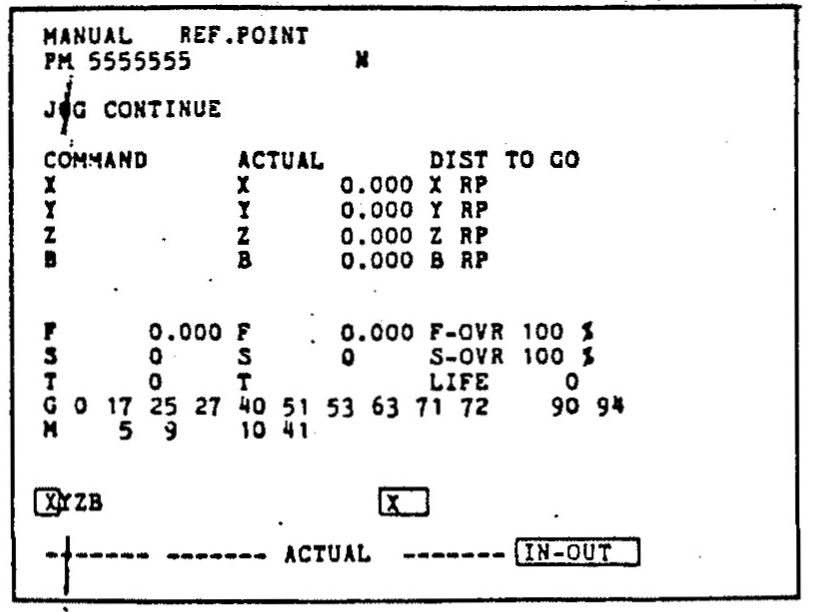
\includegraphics[width=0.7\textwidth]{manual_ref_point.jpg}
    \caption{Expected screen after successful startup}
\end{figure}

\notes

\begin{itemize}
    \item After switching on the main switch, the hardware diagnostic check of the control system is displayed on the screen first. The display automatically changes and then shows the \textbf{MANUAL} screen.
    \item In demonstration units, the \textbf{F3} function key must be pressed to display the \textbf{MANUAL} screen.
\end{itemize}

\textbf{For safety reasons}, the machine is always automatically disabled to check the \textbf{EMERGENCY STOP} circuit in the following cases:

\begin{itemize}
    \item After switching the machine’s main switch to "On".
    \item After changing the measurement unit system (see \textbf{Section 2.4}).
    \item After disabling \textbf{Diagnostic Mode} (see \textbf{Section 2.3}).
    \item After locking the machine constant memory via the locking switch located inside the machine’s electrical cabinet.
    \item After power is restored following a power failure.
\end{itemize}

\section{Referencing a Machine Axis}

The machine's axis reference points must be set:
\begin{itemize}
    \item After each startup of the machine and control system.
    \item After changing the measurement unit system (see \textbf{Section 2.4}).
    \item After disabling \textbf{diagnostic mode} (see \textbf{Section 9.3}).
    \item After locking the machine constants memory via the lock switch located in the machine’s electrical cabinet.
    \item After a power failure.
\end{itemize}

The text \textbf{REF.POINT} is displayed on \textbf{line 1} of the screen whenever the reference points for all machine axes have not been set.

In this state, only the following modes are available:
\begin{itemize}
    \item \textbf{Step-by-step operation} (see \textbf{Section 2.2}).
    \item \textbf{Data transmission} (see \textbf{Section 8}).
    \item \textbf{Manual data entry}.
\end{itemize}

\subsection{Important Notes}

When \textbf{REF.POINT} is displayed, the machine axis limit switches in the logic circuit are not yet active. This means that there is still a risk of collisions with the electromechanical \textbf{EMERGENCY STOP} limit switches.

Setting the reference point in step-by-step mode requires particular attention.

\textbf{Before setting the reference point, all risk of collision must be eliminated.}

When setting the reference point, all axes move simultaneously if they were activated before pressing the \textbf{start} button. However, it is also possible to set the reference points individually, in an arbitrary order.

\procedure

\begin{itemize}
    \iconitem {Press the \textbf{ENTER} key once for each machine axis to be referenced.}{enter.jpg}
\end{itemize}

The selected machine axes for reference setting are displayed on \textbf{line 21} of the screen:

\begin{center}
    \textbf{X-RP \quad Y-RP \quad Z-RP \quad B-RP}
\end{center}

The text \textbf{RP} appears on the screen below \textbf{DIST TO GO} for each machine axis.

\begin{itemize}
    \iconitem {Press the \textbf{START} button.}{start.jpg}
\end{itemize}

All machine axes will now move simultaneously.

\textbf{RP} is displayed under \textbf{COMMAND} during the reference setting process for each machine axis. The display disappears as soon as an axis reaches its reference point. At the same time, the value \textbf{0} appears under \textbf{DIST TO GO}, indicating that the axis is now at its reference position.

The text \textbf{REF.POINT} on \textbf{line 1} of the screen disappears once all axes have been referenced.

The deviation between the reference point and the machine's origin is displayed on the screen under \textbf{ACTUAL} for each machine axis.

At this point, the machine is operational.

\notes

Axis movements can be stopped using the \textbf{Advance Stop} or \textbf{Advance Stop and Work Spindle} buttons during the reference setting process.

In case of a collision, it is possible to \textbf{cancel the reference point} for one or more axes. Proceed as follows:

\begin{itemize}
    \iconitem {Press the \textbf{Advance Stop} or \textbf{Advance Stop and Work Spindle} button (if the reference setting has already been initialized).}{advance_stop.jpg, advance_stop_and_work_spindle.jpg}
\end{itemize}
\begin{itemize}
    \iconitem {Use the \textbf{cursor control keys (left/right)} to move the cursor to the address letter of the axis to be canceled.}{left.jpg, right.jpg}
\end{itemize}


\begin{itemize}
    \iconitem {Press the \textbf{ENTER} key.}{enter.jpg}
\end{itemize}

\vspace{.5cm}

\begin{itemize}
    \iconitem {Press the \textbf{START} button.}{start.jpg}
\end{itemize}

Only the reference points for the remaining axes can now be set.

It is also necessary to set the previously canceled reference points for the affected axes once the risk of collision has been eliminated.